% vim: set tw=78 tabstop=4 shiftwidth=4 aw ai:
\documentclass{beamer}

\usepackage[utf8x]{inputenc}		% diacritice
\usepackage[romanian]{babel}
\usepackage{color}			% highlight
\usepackage{alltt}			% highlight

% highlight; comment this out in case you don't input code source files
%\usepackage{code/highlight}		% highlight

\usepackage{hyperref}			% folosiți \url{http://...}
					% sau \href{http://...}{Nume Link}
\usepackage{verbatim}

\mode<presentation>
{ \usetheme{Berlin} }

% Încărcăm simbolurilor Unicode românești în titlu și primele pagini
\PreloadUnicodePage{200}

\title[Git Repositories]{Gestiunea repository-urilor folosind soluții Git}
\subtitle{Linux and Open Source}
\author[Răzvan Deaconescu]{Răzvan Deaconescu\\
	razvan@rosedu.org}
\date{24 februarie 2011}

\begin{document}

% Slide-urile cu mai multe părți sunt marcate cu textul (cont.)
\setbeamertemplate{frametitle continuation}[from second]

% Arătăm numărul frame-ului
%\setbeamertemplate{footline}[frame number]

\frame{\titlepage}

\frame{\tableofcontents}

% NB: Secțiunile nu sunt marcate vizual, ci doar apar în cuprins
\section{Git}

% Titlul unui frame se specifică fie în acolade, imediat după \begin{frame},
% fie folosind \frametitle
\begin{frame}{Sisteme de versionare a codului}
	\begin{itemize}		% Just like normal LaTeX
		\item aaa
		\item aaa
	\end{itemize}
\end{frame}

\begin{frame}{Git}
	\begin{itemize}
		\item aa
		\item bbb
	\end{itemize}
\end{frame}

\begin{frame}{URL-uri Git}
	\begin{itemize}
		\item aa
		\item bbb
	\end{itemize}
\end{frame}

\begin{frame}{Git peste SSH}
	\begin{itemize}
		\item aa
		\item bbb
	\end{itemize}
\end{frame}

\begin{frame}{Git peste HTTP}
	\begin{itemize}
		\item aa
		\item bbb
	\end{itemize}
\end{frame}

\begin{frame}{Protocolul Git}
	\begin{itemize}
		\item aa
		\item bbb
	\end{itemize}
\end{frame}

\begin{frame}{Rezumat}
	\begin{itemize}
		\item aa
		\item bbb
	\end{itemize}
\end{frame}

\section{Gitolite}

\frame{\tableofcontents[currentsection]}

\begin{frame}{Gitolite}
	\begin{itemize}
		\item aa
		\item bbb
	\end{itemize}
\end{frame}

\begin{frame}{Avantaje folosire Gitolite}
	\begin{itemize}
		\item aa
		\item bbb
	\end{itemize}
\end{frame}

\section{Gitweb}

\frame{\tableofcontents[currentsection]}

\begin{frame}{Gitweb}
	\begin{itemize}
		\item aa
		\item bbb
	\end{itemize}
\end{frame}

\begin{frame}{Avantaje folosire Gitweb}
	\begin{itemize}
		\item aa
		\item bbb
	\end{itemize}
\end{frame}

\section{Scenarii de utilizare}

\frame{\tableofcontents[currentsection]}

\begin{frame}{aaa}
	\begin{itemize}
		\item aa
		\item bbb
	\end{itemize}
\end{frame}

\section{Recomandări}

\begin{frame}{All is text}
	\begin{itemize}
		\item scripturi și fișiere de configurare
		\item LaTeX \& LaTeX Beamer
		\item Inkscape -- SVG, Dia -- salvare ca fișier necomprimat (format
		XML)
		\item fișiere de organizare/task-uri (Org-Mode în Emacs)
	\end{itemize}
\end{frame}

\begin{frame}{Versionare și ``diff''-ing}
	\begin{itemize}
		\item versionarea facilă a fișierelor de configurare
		(\texttt{/etc/apache2/})
		\item versionarea temelor submise (studiu de caz UPB)
		\item folosire de tag-uri pentru ani
			\begin{itemize}
				\item se lucrează peste același ``code base''
				\item nu se mai face un director pentru fiecare an
			\end{itemize}
	\end{itemize}
\end{frame}

\begin{frame}{Hook-uri}
	\begin{itemize}
		\item post-receive
		\item trimis e-mail-uri/notificări
		\item creat arhive, compilat prezentări/fișiere LaTeX, publicat
		resurse
			\begin{itemize}
				\item ușor de integrat în wiki-uri
				\item link-ul nu se schimbă, doar conținutul acestuia
			\end{itemize}
	\end{itemize}
\end{frame}

\section{Încheiere}

\begin{frame}{Resurse utile}
	\begin{itemize}
		\item \url{http://git-scm.com/}
		\item \url{http://progit.org/}
		\item \url{http://github.com/sitaramc/gitolite}
		\item \url{https://git.wiki.kernel.org/index.php/Gitweb}
	\end{itemize}
\end{frame}

\begin{frame}{Întrebări}
%	\begin{columns}
%		\begin{column}[l]
%			\begin{itemize}
%				\item aa
%				\item bb
%			\end{itemize}
%		\end{column}
%		\begin{column}[l]
%			\begin{figure}
%				\centering
%				\includegraphics{img/question-mark}
%			\end{figure}
%		\end{column}
%	\end{columns}
\end{frame}

\end{document}
